\section{L'implémentation de l'interface graphique}\label{sec:l'implementation-de-l-interface-graphique}
\subsection{Bibliothèques utilisées (SFML)}\label{subsec:sfml}
SFML (\textit{Simple and Fast Multimedia Library}) est une bibliothèque C++ qui permet de créer des applications multimédia.
Elle est particulièrement adaptée pour le développement de jeux vidéo et d'applications graphiques.
Elle fournit des fonctionnalités pour la gestion des fenêtres, le rendu graphique, la gestion des événements, le son et la communication réseau.
En interne, elle s'appuie sur OpenGL, une API bas niveau, ce qui permet d'obtenir d'excellentes performances graphiques tout en restant simple d'utilisation.

SFML a été choisie pour plusieurs raisons :
\begin{itemize}
    \item \textbf{Simplicité d'utilisation} : Elle permet de se concentrer sur la logique applicative plutôt que sur des détails techniques complexes.
    \item \textbf{Documentation et communauté} : Sa documentation\cite{documentationSFML} est complète et une large communauté offre de nombreux exemples et ressources.
    \item \textbf{Multiplateforme} : La compatibilité avec Windows, Linux et macOS permet de développer l'application sans penser à la portabilité.
\end{itemize}

\subsection{Architecture de l'interface graphique}\label{subsec:architecture-de-l-interface-graphique}
\subsubsection{Organisation modulaire du code}\label{subsubsec:organisation-modulaire-du-code}
Pour garantir la lisibilité et la maintenabilité du code, l'interface graphique a été conçue de manière modulaire.
Chaque fonctionnalité est encapsulée dans une classe dédiée, permettant ainsi une séparation claire des responsabilités.
Par exemple, la gestion du véhicule, du circuit, des indicateurs de débogage sont traitées dans des modules distincts.
Cette approche facilite également l'ajout de nouvelles fonctionnalités sans modifier la structure existante.

\subsubsection{Présentation des classes principales}\label{subsubsec:presentation-des-classes-principales}
Plusieurs classes clés interagissent pour offrir une interface graphique cohérente et fluide.

\paragraph[Game]{La Classe \textbf{Game}}\label{par:class_game}
C'est la classe principale du projet, elle orchestre l'application.
Elle initialise la fenêtre SFML, configure les vues (Game View et HUD View), gère le cycle de vie de la simulation (mise à jour, gestion des événements et rendu) et coordonne les interactions entre les différents modules.

Elle contient 3 fonctions principales :
\begin{lstlisting}[style=CStyle, label={lst:game_class}]
    void update();
    void render() const;
    void manageEvents();
\end{lstlisting}
Chaque fonction est appelée une fois par itération de la boucle principale de l'application et donc par image générée.
Voici leurs rôles respectifs :
\begin{itemize}
    \item \texttt{update()}, met à jour l'état de l'application en fonction du temps écoulé et des événements utilisateurs.
    \item \texttt{render()}, effectue le rendu graphique de la scène actuelle.
    \item \texttt{manageEvents()}, gère les événements à l'intérieur de l'application (clavier, souris), elle est appelée dans la fonction \texttt{update()}.
\end{itemize}

\paragraph[Circuit]{La Classe \textbf{Circuit}}
Elle représente, comme son nom l'indique, un circuit de conduite.
Elle est composée de différents segments de routes (comme une petite ligne droite, un petit virage, un grand virage, \dots).
Chaque segment est une portion de route qui peut être droite ou courbe, et la classe gère la connexion entre ces segments pour former une impression de circuit continue au niveau de l'affichage graphique. \\
Son fonctionnement interne permet, de l'extérieur de la classe, de simplifier la création de la route.
Il suffit de rajouter des segments de route dans le circuit en précisant l'angle à donner à la texture et s'il faut lui appliquer un effet mirroir, et la classe se charge de les relier entre eux.

L'extrait de code suivant permet de réaliser ce bout de circuit (fig.~\ref{fig:example_circuit_1}) :
\begin{lstlisting}[style=CStyle, label={lst:code_circuit}]
Circuit circuit;
circuit.setOrigin(ResourceType::Value::SEGMENT_SMALL_STRAIGHT);
circuit.join(ResourceType::Value::SEGMENT_S_TURN);
circuit.join(ResourceType::Value::SEGMENT_MEDIUM_TURN);
circuit.join(ResourceType::Value::SEGMENT_LARGE_TURN, 90);
circuit.join(ResourceType::Value::SEGMENT_U_TURN, 180);
circuit.join(ResourceType::Value::SEGMENT_U_TURN, 0, false, true);
circuit.join(ResourceType::Value::SEGMENT_LONG_STRAIGHT, 180);
\end{lstlisting}

\begin{figure}[h]
    \centering
    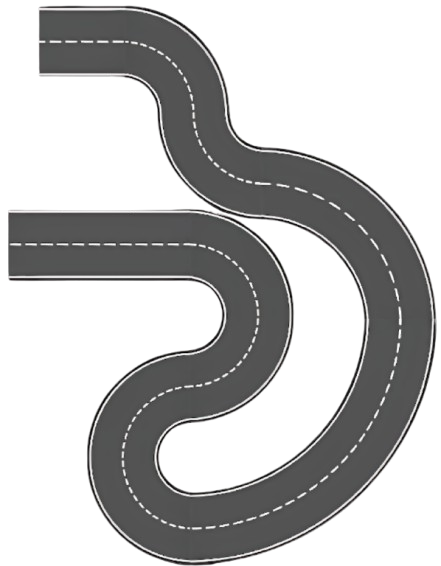
\includegraphics[width=0.5\textwidth]{resources/example_circuit_1}
    \caption{Exemple de circuit pouvant être généré grâce à la classe Circuit}
    \label{fig:example_circuit_1}
\end{figure}

\paragraph[Car]{La classe \textbf{Car}}
Cette classe encapsule la classe \texttt{Vehicle} (voir section \ref{sec:l'implementation-de-la-physique-/-modelisation-d'un-systeme-de-dynamique-de-vehicule}).
L'interaction entre les deux classes \texttt{Car} et \texttt{Vehicle} est présentée à la section\ref{subsubsec:interactions-entre-l-interface-graphique-et-la-partie-physique}.
Elle calcule la ligne de prédiction de la trajectoire du véhicule et gère l'affichage du véhicule.

Lors du développement de la ligne de prédiction de trajectoire, nous avons rencontré un problème.
Le calcul prend en paramètre un delta de temps qui correspond au temps entre la dernière image et l'image actuelle.
Ce delta de temps est très volatile et peut varier du simple au double, ce qui cause de grosses différences de longueur de la ligne de prédiction et provoque une impression de scintillement.

Pour résoudre ce problème, nous avons décidé de récupérer le delta de temps médian sur les 1000 dernières images.

\begin{lstlisting}[style=CStyle, label={lst:code_dequeue_dt}]
std::deque<float> dtBuffer;
const size_t max_dt_buffer_size = 1000;
float updateAndGetMedian(const float dt) {
    dtBuffer.push_back(dt);
    if (dtBuffer.size() > max_dt_buffer_size) {
        dtBuffer.pop_front();
    }
    std::vector tmp(dtBuffer.begin(), dtBuffer.end());
    const auto mid = tmp.begin() + tmp.size() / 2;
    std::nth_element(tmp.begin(), mid, tmp.end());
    return *mid.base();
}
\end{lstlisting}

La complexité de la fonction \texttt{updateAndGetMedian(const float dt)} est en \( O(n) \).
Voici le détail de la complexité :
\begin{itemize}
    \item \texttt{push\_back(dt)} : \( O(1) \)\cite{cpp_reference_push_back} pour ajouter un élément à la fin de la deque.
    \item \texttt{pop\_front()} : \( O(1) \)\cite{cpp_reference_pop_front} pour retirer le premier élément de la deque.
    \item \texttt{std::vector tmp(dtBuffer.begin(), dtBuffer.end())} : \( O(n) \)\cite{cpp_reference_vector} pour copier la deque dans un vecteur.
    \item \texttt{std::nth\_element(tmp.begin(), mid, tmp.end())} : \( O(n) \)\cite{cpp_reference_std_nth_element} pour trier le vecteur jusqu'à l'élément médian.
\end{itemize}

On a utilisé la fonction \texttt{std::nth\_element()}\cite{cpp_reference_std_nth_element} car elle permet de ne pas trier l'ensemble du vecteur tout en plaçant l'élément médian à la bonne position dans le \texttt{std::vector}\cite{cpp_reference_vector}.
Au départ, nous avions utilisé la fonction \texttt{std::sort()}, qui trie un vecteur complet, mais sa complexité aurait été en \( O(n \log n) \)\cite{cpp_reference_std_sort}, ce qui est moins optimal étant donné que la ligne de prédiction est recalculée à chaque image.


\subsubsection{Les ressources}\label{subsubsec:gestion-des-ressources}
\paragraph{Type de ressources}
Dans le projet, nous avons principalement deux types de ressources :
\begin{itemize}
    \item Les \textbf{Textures} : Utilisées pour le rendu graphique des segments de route et du véhicule.
    \item Les \textbf{Polices de caractères} : Utilisées pour le rendu du texte dans l'interface graphique.
\end{itemize}

\paragraph{Les textures}
Au sein de la librairie SFML, une image est représentée avec une classe \texttt{sf::Texture}\cite{sfml_sf_texture} qui contient la représentation en mémoire des pixels de l'image.
Chaque texture (ou image) correspond à une entrée dans une enum \texttt{ResourceType::Value} qui permet de les identifier de manière unique, cela concerne les segments de route ainsi que l'image de la voiture.
Cette enum est définie dans le fichier \texttt{resource\_type.h} et contient les valeurs suivantes :
\begin{itemize}
    \item \texttt{SEGMENT\_SMALL\_STRAIGHT} : Une petite ligne droite.
    \item \texttt{SEGMENT\_LONG\_STRAIGHT} : Une grande ligne droite.
    \item \texttt{SEGMENT\_SMALL\_TURN} : Un virage moyen.
    \item \texttt{SEGMENT\_MEDIUM\_TURN} : Un virage moyen.
    \item \texttt{SEGMENT\_LARGE\_TURN} : Un virage large.
    \item \texttt{SEGMENT\_S\_TURN} : Un virage en S (plus communément appelé une chicane)
    \item \texttt{SEGMENT\_U\_TURN} : Un virage en U\@.
    \item \texttt{CAR} : La texture de la voiture.
\end{itemize}

\paragraph{La police d'écriture}
La police d'écriture utilisée dans le projet est la \textit{DejaVu Sans Mono}.
Pour plus de portabilité de notre code, nous avons décidé de l'inclure dans le projet.

Nous avons généré un fichier C++ contenant les données binaires de la police \textit{DejaVu Sans Mono} en utilisant la commande suivante :
\begin{lstlisting}[style=BashStyle,label={lst:generation_dejavusansmonottf_h}]
xxd -i DejaVuSansMono.ttf > dejavu_sans_mono_ttf.cpp
\end{lstlisting}
Cette commande convertit le fichier binaire de la police d'écriture en un tableau de bytes C++ que nous pouvons inclure directement dans notre projet.
Le fichier généré contient deux éléments :
\begin{itemize}
    \item Un tableau de bytes contenant les données binaires de la police d'écriture.
    \item La taille du tableau de bytes.
\end{itemize}
Cette solution, trouvée sur Stack Overflow\cite{stackoverflow_embed_font}, nous permet d'intégrer la police directement dans le binaire de l'application, assurant ainsi une portabilité maximale.

\paragraph{Gestionnaire de ressources}
Nous avons fait le choix de séparer la gestion de ces deux types de ressources en deux classes différentes étant donné leurs utilisations différentes.
La classe \texttt{TextureManager} gère le chargement des images dans la mémoire de l'application.
Lorsque l'on a besoin d'utiliser une \texttt{sf::Texture}\cite{sfml_sf_texture}, on fait appel à la méthode \texttt{TextureManager::getTexture()} qui prend en paramètre un \texttt{ResourceType::Value} et renvoie un pointeur vers la texture correspondante.
Deux cas sont possibles :
\begin{itemize}
    \item La texture n'a jamais été demandée depuis le début de l'exécution, elle est donc chargée depuis le disque dur et stockée dans une \texttt{std::unordered\_map<ResourceType::Value, sf::Texture>}\cite{cpp_reference_std_unordered_map}.
    \item La texture a déjà été chargée, une référence vers la \texttt{sf::Texture}\cite{sfml_sf_texture} correspondante est récupérée puis renvoyée.
    Ici, on utilise une référence et non une copie, car aucun traitement n'est fait directement sur l'objet en mémoire.
\end{itemize}
Ce système permet de ne charger qu'une seule fois une texture et de la réutiliser à chaque fois qu'elle est demandée, ce qui limite grandement l'utilisation de la mémoire.

Pour ce qui est des polices de caractères, la classe \texttt{FontManager} fonctionne de manière similaire, mais nous n'utilisons qu'une seule police de caractères pour l'ensemble de l'application.
Lors de la création de l'objet, la police est chargée depuis le disque dur et stockée dans un pointeur (\texttt{std::unique\_ptr<sf::Font>}\cite{cpp_reference_std_unique_ptr}) dans un attribut de la classe.

\paragraph{Connexion des segments de routes}
En interne, la texture d'un segment de route est représentée par une structure \texttt{RoadTexture} définie comme suit :

\begin{lstlisting}[style=CStyle,label={lst:struct_roadtexture}]
struct RoadTexture {
    const sf::Texture *texture = nullptr;
    sf::Sprite sprite;
    sf::Vector2f point1;
    sf::Vector2f point2;
};
\end{lstlisting}

Elle contient 4 éléments :
\begin{itemize}
    \item \texttt{texture} : Un pointeur vers la texture de la route chargée par le \texttt{TextureManager}.
    \item \texttt{sprite} : Le \gls{sprite} associé à la texture, utilisé pour le rendu.
    \item \texttt{point1} et \texttt{point2} : Deux positions relatives à la texture représentant les points de connexion entre deux segments de route.
\end{itemize}

Lorsque l'on ajoute un nouveau segment via la fonction \texttt{join()}, le processus se déroule comme suit :

\begin{enumerate}
    \item \textbf{Récupération du segment précédent :}
    La fonction commence par récupérer le dernier segment inscrit dans le circuit (via \texttt{segments.back()}).
    Ce segment précédent fournit la position finale (stockée dans \texttt{realPoint2}) qui sera utilisée comme point de départ pour le nouveau segment.

    \item \textbf{Génération et configuration de la texture :}
    À l'aide de la fonction \\\texttt{generate\_road\_texture()}, on crée la texture du nouveau segment en passant par le gestionnaire de textures, tout en tenant compte des éventuelles opérations de mirroring (horizontal et/ou vertical).
    Ensuite, la texture (via son \gls{sprite}) est mise à l’échelle en fonction du facteur de zoom courant (\texttt{game->getZoomFactor()}) pour garantir une cohérence visuelle.

    \item \textbf{Alignement du nouveau segment :}
    Pour assurer la continuité, l'origine du \gls{sprite} du nouveau segment est fixée au point de connexion de départ (\texttt{road\_texture.point1}).
    Le \gls{sprite} est ensuite positionné exactement à l'endroit où se termine le segment précédent (\texttt{fromPoint2}).
    Cela garantit que le nouveau segment démarre précisément à la fin du précédent.

    \item \textbf{Calcul du point de raccord final avec rotation :}
    Afin de déterminer la position finale du nouveau segment, on calcule un décalage à partir de sa position initiale.
    \begin{itemize}
        \item On commence par obtenir la position globale du \gls{sprite} via \\\texttt{spr->getGlobalBounds().getPosition()}.
        \item Ce point est ensuite ajusté en y ajoutant l'offset correspondant à \\\texttt{road\_texture.point2} (après application du zoom), ce qui permet d'estimer où devrait se trouver la fin du segment sans rotation.
        \item Ensuite, la fonction \texttt{rotatePoint()} est utilisée pour faire pivoter ce point autour du point de raccord initial (\texttt{fromPoint2}) selon l'angle spécifié.
        Le résultat est le nouveau point final (\texttt{rotatedPoint}) qui définit l'orientation et l'emplacement du bout du segment après application de la rotation.
    \end{itemize}

    \item \textbf{Application de la rotation et ajout du segment :}
    Une fois le point final calculé, le \gls{sprite} est tourné à l’angle désiré (en veillant à appliquer la rotation après le calcul afin d’éviter une double rotation).
    Finalement, le segment (contenant la texture, la rotation, le point de départ et le point final calculé) est ajouté à la liste des segments du circuit.
\end{enumerate}

Ce mécanisme garantit que chaque segment est correctement positionné par rapport à celui qui le précède, assurant ainsi une continuité visuelle du circuit.
L'utilisation de fonctions telles que \texttt{rotatePoint()} permet également de gérer facilement les changements d'orientation, ce qui est crucial pour modéliser des virages et des segments courbes.
De plus, le support des opérations de mirroring permet de varier les configurations de segments tout en réutilisant la même texture, offrant ainsi une plus grande flexibilité dans la conception du circuit.


% TODO Si changé, modifier le paragraph Car.
\subsubsection{Interactions entre l'interface graphique et la partie physique}\label{subsubsec:interactions-entre-l-interface-graphique-et-la-partie-physique}
Bien que l'interface graphique et la simulation physique soient implémentées dans des modules distincts, leur intégration est cruciale pour offrir une expérience fluide et cohérente. Plusieurs mécanismes d'interaction ont été mis en place :

\begin{itemize}
    \item \textbf{Mise à jour en temps réel :} La classe \texttt{Car} interroge en continu le modèle physique (géré par la classe \texttt{Vehicle}) pour récupérer les données essentielles telles que la position, la vitesse, l'orientation et la trajectoire prédictive.
    Ces informations sont immédiatement utilisées pour actualiser le \gls{sprite} du véhicule ainsi que la ligne de prédiction affichée.
    \item \textbf{Synchronisation et cohérence visuelle :} Les calculs physiques (notamment via l'intégration numérique de la dynamique du véhicule) génèrent des états qui sont transmis à l'interface graphique.
    Cela garantit que l'affichage du véhicule, de ses effets et de sa trajectoire reflète précisément l'évolution dynamique simulée.
    \item \textbf{Traçage de la trajectoire prédictive :} En parallèle, la classe \texttt{Car} calcule une trajectoire prédictive basée sur les itérations futures de la dynamique physique.
    Cette trajectoire, rendue à l'aide d'un \texttt{sf::VertexArray}\cite{sfml_sf_vertexarray}, permet à l'utilisateur de visualiser l'impact des commandes de conduite sur le comportement futur du véhicule.
\end{itemize}

Ces interactions étroites entre la partie physique et l'interface graphique permettent non seulement une synchronisation efficace entre les calculs et le rendu, mais également une meilleure compréhension et un contrôle précis du comportement dynamique du véhicule.


\subsection{Composants et fonctionnalités}\label{subsec:composants-et-fonctionnalites}

\subsubsection{Visualisation des informations dynamiques}\label{subsubsec:visualisation-des-informations-dynamiques}

\paragraph{Mode de Debug}
Le mode Debug (Figure~\ref{fig:debug_mode}) offre une visualisation en temps réel de diverses informations physiques (vitesse, forces, angles, etc.).
Cette fonctionnalité, représentée par la classe \texttt{DebugMode}, est particulièrement utile pour le débogage et l'analyse du comportement du véhicule.
Elle permet de suivre l'évolution des paramètres physiques au fil du temps, facilitant ainsi l'identification de problèmes potentiels ou d'anomalies dans le comportement dynamique.
Il est possible de l'activer ou de la désactiver à l'aide de la touche \texttt{F3}.
Cette classe contient un attribut \texttt{std::vector<sf::Text>}\cite{cpp_reference_vector} qui contient les textes à afficher dans la HUD View.

On ajoute un texte à la liste en utilisant la méthode \texttt{addLine()} qui prend en paramètre le texte à afficher, la position et la couleur du texte.
Cette méthode rajoute aussi un fond semi-transparent au texte pour le rendre plus lisible lorsque le fond est trop chargé.

\begin{lstlisting}[style=CStyle, label={lst:code_addline}]
void DebugMode::addLine(const std::string &content, const unsigned int size, const sf::Color &color) {
    sf::Text text;
    text.setFont(font);
    text.setCharacterSize(size);
    text.setFillColor(color);
    text.setString(content);

    sf::RectangleShape background;
    background.setSize(sf::Vector2f(text.getLocalBounds().width, text.getLocalBounds().height + 6.25f));
    background.setFillColor(sf::Color(64, 64, 64, 255/2));

    texts.push_back(text);
    backgrounds.push_back(background);
}
\end{lstlisting}
\begin{figure}[H]
    \centering
    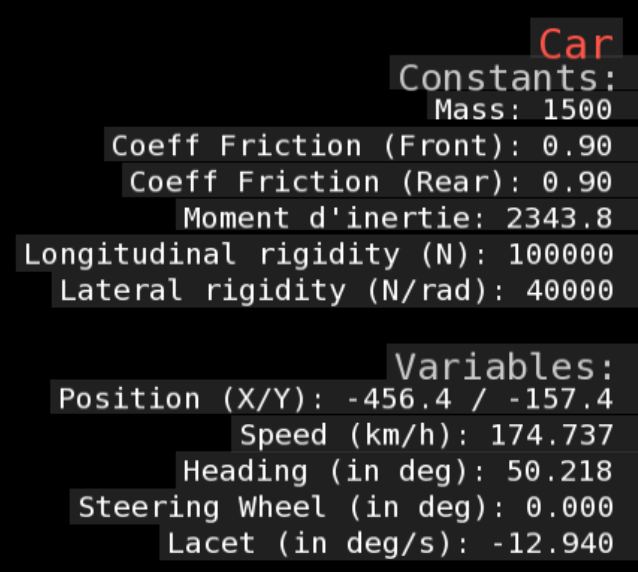
\includegraphics[width=0.5\textwidth]{resources/example_debug_mode_1}
    \caption{Exemple de mode Debug}
    \label{fig:debug_mode}
\end{figure}

\paragraph{Compteur de FPS}
La classe \texttt{FPSCounter} affiche le nombre de frames par seconde dans la HUD View, permettant ainsi de surveiller la fluidité de l'application.
Elle nous permet, tout au long du développement, de remarquer si une fonctionnalité que l'on vient d'implémenter est trop gourmande en ressources et de l'optimiser en conséquence.

Pour calculer le nombre d'images par seconde, on compte le nombre d'images générées en une seconde.
La classe contient, parmi ses attributs, un compteur d'image \texttt{frameCount} et un accumulateur de temps \texttt{timeAccumulator}.
\begin{lstlisting}[style=CStyle, label={lst:code_fpscounter}]
void FPSCounter::update(const float dt) {
    timeAccumulator += dt;
    frameCount++;
    if (timeAccumulator >= 1.f) {
        currentFPS = frameCount;
        frameCount = 0;
        timeAccumulator = 0.f;
        text.setString("FPS: " + std::to_string(currentFPS));
    }
}
\end{lstlisting}
Le paramètre \texttt{dt} est le delta de temps entre la dernière image et l'image actuelle.

À chaque nouvelle image et donc à chaque appel de la fonction \texttt{update()} (paragraphe sur la classe Game :~\ref{par:class_game}) de la classe \texttt{Game}, on appelle la fonction \texttt{update()} de la classe \texttt{FPSCounter} en lui passant le delta de temps.
On ajoute le delta de temps à l'accumulateur de temps et on incrémente le compteur d'image.
Lorsque l'accumulateur de temps dépasse 1 seconde, on met à jour le nombre d'images par seconde et on remet le compteur d'image et l'accumulateur de temps à zéro.

\subsubsection{Affichage de la trajectoire et prédictions}\label{subsubsec:affichage-de-la-trajectoire-et-predictions}
Dans notre simulateur, la trajectoire prédictive joue un rôle clé en offrant à l'utilisateur une estimation visuelle de l'évolution future du véhicule en fonction de son état dynamique actuel.
Cette fonctionnalité permet non seulement de mieux comprendre l'impact immédiat des commandes de conduite, mais aussi d'anticiper les conséquences de ces actions sur le comportement global du véhicule.

\begin{figure}[H]
    \centering
    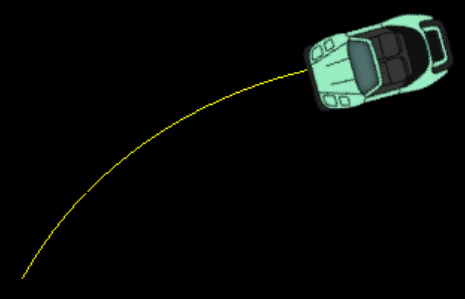
\includegraphics[width=0.5\textwidth]{resources/example_prediction_line_1}
    \caption{Exemple de ligne de prédiction des mouvements.}
    \label{fig:prediction_line}
\end{figure}

\paragraph{Calcul de la trajectoire prédictive}
Pour obtenir la trajectoire prédictive, nous simulons l'évolution du véhicule en itérant la dynamique physique sur plusieurs pas de temps à chaque image.
La fonction \texttt{computePredictionLine} procède de la manière suivante :
\begin{itemize}
    \item Le delta de temps utilisé pour ces itérations est déterminé de manière robuste grâce à la fonction \texttt{updateAndGetMedian} (définition dans le paragraphe \textbf{La classe Car} :~\ref{lst:code_dequeue_dt}), qui calcule la médiane des deltas de temps récents afin de lisser les variations liées à la volatilité du temps entre images.
    \item À partir de l'état courant du véhicule, la dynamique est simulée en appliquant un schéma d'intégration numérique (ici la méthode Runge-Kutta d'ordre 4, ou RK4).
    Pour chaque itération, la nouvelle position et l'orientation sont calculées et stockées dans un tableau.
    \item Ces points, une fois convertis en coordonnées écran via le facteur de conversion (par exemple, \texttt{METER\_TO\_PIXEL}), représentent la trajectoire future du véhicule.
\end{itemize}

\paragraph{Tracé en temps réel via les données issues de la simulation}
L'affichage de cette trajectoire prédictive est géré en temps réel grâce à un objet \texttt{sf::VertexArray}\cite{sfml_sf_vertexarray} configuré en mode \texttt{LineStrip}.
À chaque frame :
\begin{itemize}
    \item Les points prédits sont recalculés et le \texttt{VertexArray} est mis à jour pour refléter le chemin futur du véhicule.
    \item La visualisation dynamique permet à l'utilisateur de voir immédiatement l'effet des commandes de conduite sur la trajectoire prévue, offrant ainsi un retour visuel direct sur l'évolution de l'état du véhicule.
    \item Cette approche interactive aide également à identifier et à ajuster les paramètres du modèle physique en observant comment de petites modifications influent sur le comportement prévisionnel.
\end{itemize}

\subsubsection{Gestion des événements utilisateurs}\label{subsubsec:gestion-des-evenements-utilisateurs}
La gestion des interactions se fait principalement via la méthode \texttt{manageEvents()} de la classe \texttt{Game} :
\begin{itemize}
    \item \textbf{Clavier} : La touche F active/désactive le compteur de FPS, F3 bascule le mode Debug, F5 réinitialise la position du véhicule et ESC ferme l'application.
    \item \textbf{Souris} : Le défilement de la molette permet d'ajuster le niveau de zoom sur la Game View, offrant ainsi à l'utilisateur la possibilité de mieux suivre le véhicule ou d'obtenir une vue d'ensemble du circuit.
\end{itemize}
Ce système d'événements assure une interactivité réactive et une expérience utilisateur intuitive.

\subsection{Optimisation du rendu et de l'affichage}\label{subsec:optimisation-du-rendu-et-de-l-affichage}
\subsubsection{Gestion des vues}\label{subsubsec:gestion-des-vues}
Dans le simulateur, on peut distinguer deux vues :
\begin{itemize}
    \item \textbf{Game View} : C'est la vue principale où le circuit et le véhicule sont affichés.
    Elle est centrée sur le véhicule, offrant une perspective immersive de la conduite.
    \item \textbf{HUD View} : Cette vue affiche des informations supplémentaires, telles que le compteur de FPS et les données de débogage.
\end{itemize}

C'est ce qui nous permet de suivre le véhicule avec la \og caméra \fg{} sans que cela n'affecte les informations affichées dans la HUD View.

\subsubsection{Optimisations mises en œuvre}\label{subsubsec:optimisations-mises-en-oeuvre}
Afin d'assurer une fluidité optimale du simulateur, plusieurs optimisations ont été mises en œuvre :
\begin{itemize}
    \item \textbf{Calcul du circuit} : Le circuit est calculé une première fois, puis stocké dans un tableau de segments de route (\texttt{std::vector<RoadSegment>}\cite{cpp_reference_vector}).
    Lorsque le circuit a besoin d'être recalculé, par exemple lors d'une modification du zoom, un appel à la méthode \texttt{needUpdate()} le définit comme obsolète, et il est recalculé lors de la prochaine itération de la boucle principale.
    \item \textbf{Utilisation de Vertex Arrays} : Le tracé de la trajectoire est réalisé à l'aide d'un \texttt{sf::VertexArray}\cite{sfml_sf_vertexarray}, ce qui permet de dessiner une série de points connectés en un seul appel de rendu.
    \item \textbf{Gestion efficace de la vue} : La Game View est ajustée dynamiquement en se recentrant sur le véhicule, minimisant ainsi les recalculs inutiles et garantissant que seul le contenu pertinent est redessiné.
\end{itemize}

\subsection{Perspectives d'amélioration et évolutions futures}\label{subsec:perspectives-d-evolution}
Bien que l'interface graphique actuelle réponde aux besoins du projet, plusieurs axes d'amélioration ont été identifiés pour de futures itérations :
\begin{itemize}
    \item \textbf{Effets visuels avancés} : L'ajout d'animations, d'effets de particules ou de transitions fluides pourrait enrichir l'expérience utilisateur.
    \item \textbf{Interface utilisateur interactive} : La mise en place de menus interactifs, d'options de configuration en temps réel ou d'indicateurs graphiques plus sophistiqués permettrait de personnaliser davantage la simulation.
    \item \textbf{Optimisation multi-threading} : La séparation des calculs physiques et du rendu graphique sur des threads distincts pourrait améliorer la réactivité et la fluidité de la simulation sur des systèmes multi-cœurs.
    \item \textbf{Extensions de la HUD View} : Intégrer davantage d'informations (comme des graphiques temps réel ou des indicateurs de performance détaillés) pourrait offrir un meilleur retour utilisateur.
\end{itemize}
